\documentclass[a4paper, 12pt]{article}
\usepackage[utf8]{inputenc}
\usepackage[margin=1.25in]{geometry}
\usepackage[style=ieee]{biblatex}
\usepackage{hyperref}
\usepackage{lipsum}
\usepackage{graphicx}
\usepackage{float}
\graphicspath{ {./images/} }

\title{\textbf{EEE 586 Term Project Proposal}\\\Large \textit{Text Classification with Graph Neural Networks}}
\author{Arda Can Aras, Tuna Alikaşifoğlu}
\date{\today}
\bibliography{bibliography}
\hypersetup{
    colorlinks=true,
    allcolors=black
}

\begin{document}
% \begin{titlepage}
\maketitle
%     \thispagestyle{empty}
% \end{titlepage}

\section{Aim \& Purpose}
In this project we will work on sentiment classification problem. The purpose of this project is to design a graph neural network model to correctly classify the sentiments of the tweets in the dataset.

\section{Inspiration}
There are only a limited number of studies that have explored the Graph Convolutional Neural Networks. The vanilla Text GCN model in~\autocite{yao2018graph} showed that it can surpass most of the state-of-the-art models without any external word embeddings of knowledge on the benchmark datasets. Therefore, there is still room to improve on this structure and obtain better results.

\section{Approaches and Methods}
The aim of this project is to obtain a novel graph based model that can classify 20 different categories. Text GCN model in the~\autocite{yao2018graph} will be the baseline model for this project and we will try to adapt the structure to our own problem. Furthermore, we also want to develop novel structures to even increase the performance of this model.

\section{Literature Review}
The related text classification with GNNs are~\autocite{yao2018graph,kipf2017semisupervised,peng2019hierarchical}. Also there is an architecture which uses attention mechanism with Graph Neural Networks~\autocite{velickovic2018graph}.

\section{Dataset}
The dataset that will be used in this project is TweetEval. It consists of seven heterogeneous tasks in Twitter, all framed as multi-class tweet classification. These tasks are irony, hate, offensive, stance, emoji, emotion, emotion and sentiment. In this project emoji multi-class classification tasks will be investigated. There are a total of 20 different emojis which represent the text. Datasets can be found here~\autocite{tweeteval}.

\section{Gantt Chart}
The Gantt chart of the work packages are provided in~\autoref{fig:gantt}.
\begin{figure}[H]
    \centering
    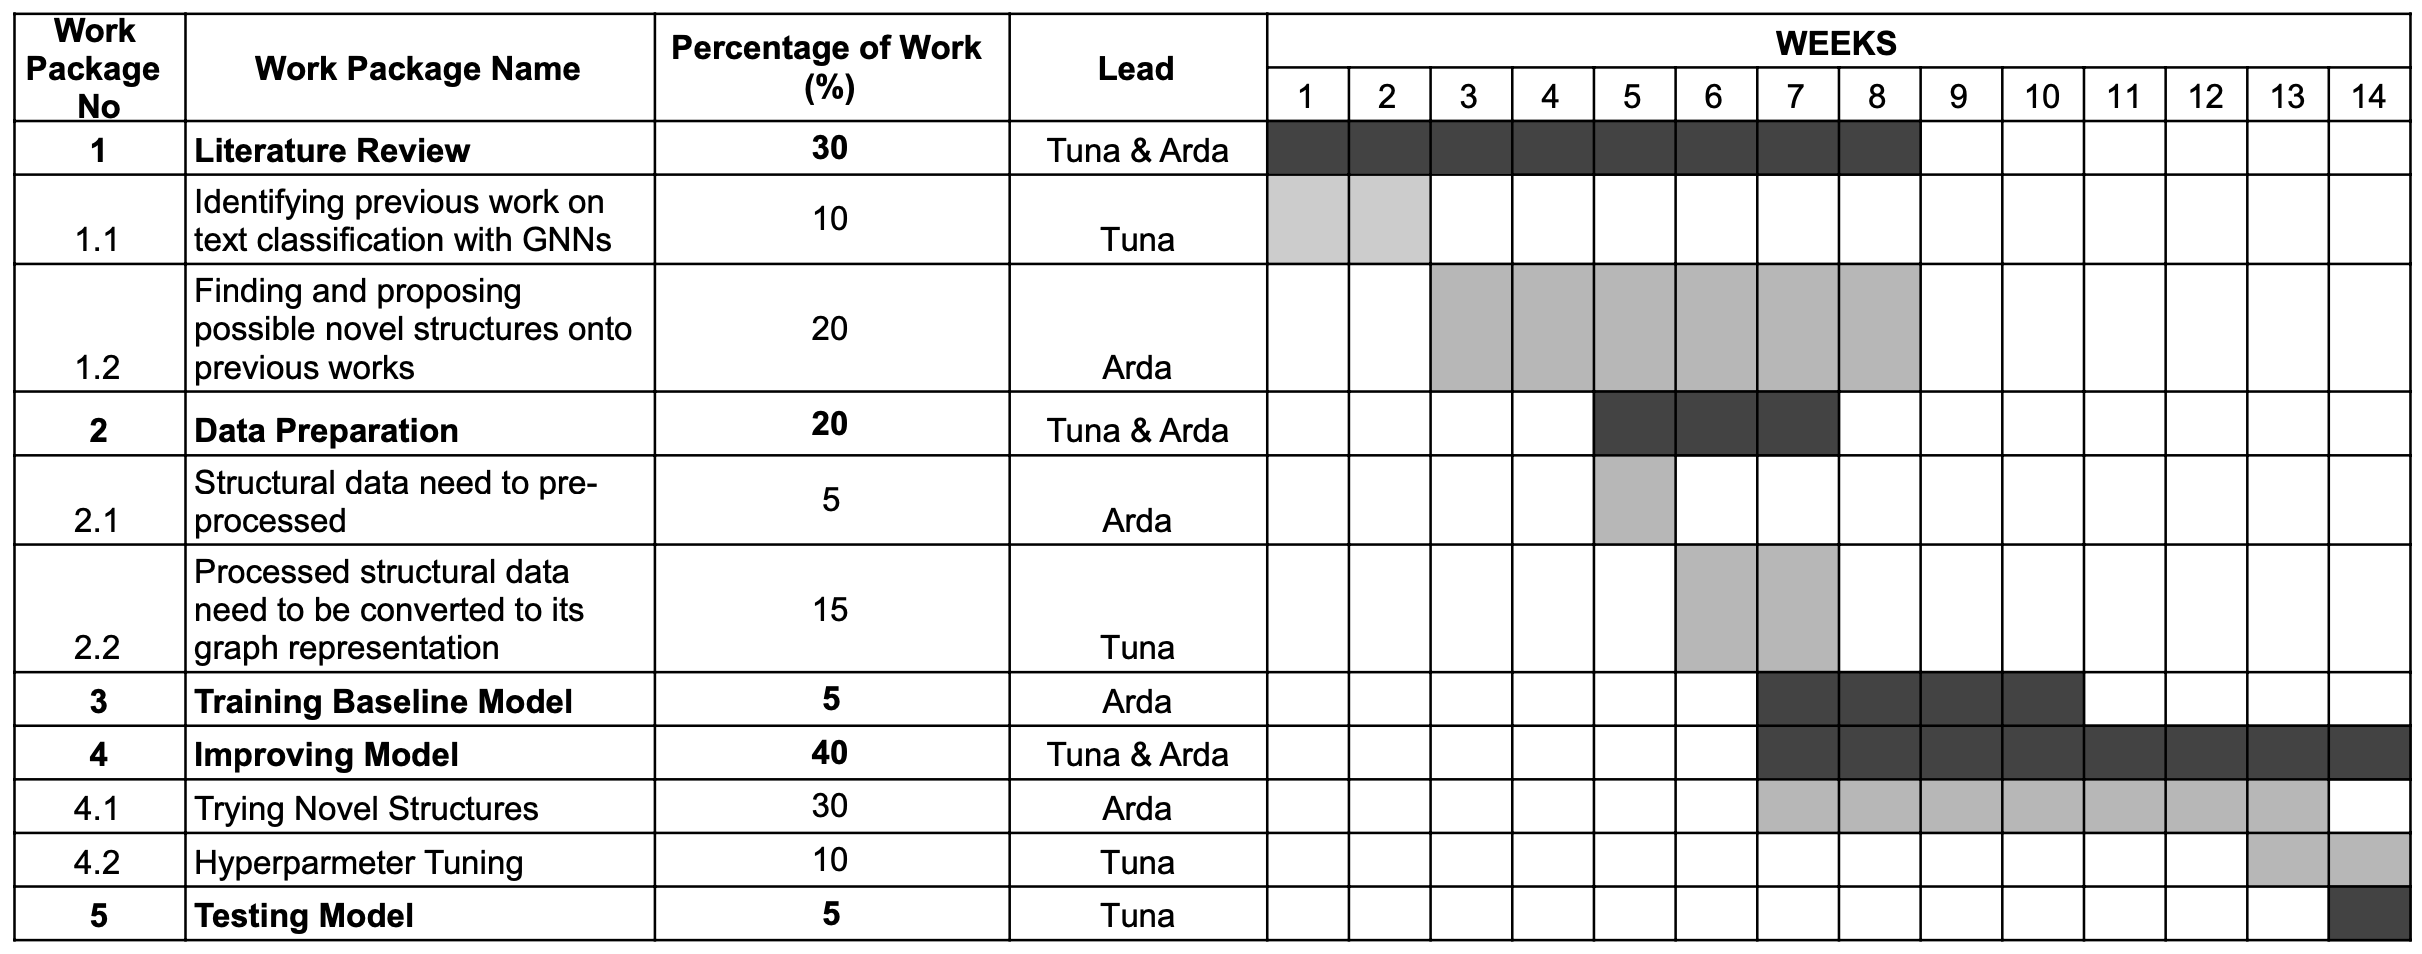
\includegraphics[width=\linewidth]{gann.png}
    \caption{Gantt Chart}
    \label{fig:gantt}
\end{figure}

\printbibliography{}
\end{document}
